\documentclass[12pt]{article} 
\usepackage[french]{babel}
\usepackage{geometry} 
\geometry{a4paper} 


% \begin{center}
% \includegraphics[width=300px]{1_sinusoide.jpg}
% \end{center}
% \vspace{0.5cm}

\usepackage[utf8]{inputenc}
\usepackage{graphicx}
\usepackage{eso-pic}
\usepackage{listings}
\usepackage{caption}
\newcommand{\q}[1]{``#1''}


\usepackage{color}
\definecolor{lightgray}{rgb}{.9,.9,.9}
\definecolor{darkgray}{rgb}{.4,.4,.4}
\definecolor{purple}{rgb}{0.65, 0.12, 0.82}
\definecolor{lightpurple}{rgb}{0.8,0.8,1}
\definecolor{javared}{rgb}{0.6,0,0}
\definecolor{javagreen}{rgb}{0.25,0.5,0.35}
\definecolor{javapurple}{rgb}{0.5,0,0.35}
\definecolor{javadocblue}{rgb}{0.25,0.35,0.75}

\lstset{
  language=Java,
	basicstyle=\ttfamily,
	keywordstyle=\color{javapurple}\bfseries,
	stringstyle=\color{javared},
	commentstyle=\color{javagreen},
	morecomment=[s][\color{javadocblue}]{/**}{*/},
	numbers=left,
	numberstyle=\tiny\color{black},
	stepnumber=2,
	numbersep=10pt,
	tabsize=4,
	showspaces=false,
	showstringspaces=false
}


% \begin{minipage}[b]{0.4\textwidth}
% 	\includegraphics[width=\textwidth]{index.png}
% 	\captionof{figure}{page d'accueil}
% \end{minipage}
% \hfill
% \begin{minipage}[b]{0.4\textwidth}
% 	\includegraphics[width=\textwidth]{profil.png}
% 	\captionof{figure}{page de profil}
% \end{minipage}



\author{Celestin Vallois, Maxime Deranty \& Baaziz Mohamed-Lamine}
\title{SR03 - Projet 2 \\  Application web JEE}

\begin{document}

\maketitle

\vspace{2cm}

\begin{center}
	
\includegraphics[width=300px]{java-jee-logo.jpg}
\end{center}

\newpage
\tableofcontents
\newpage

\part*{Introduction}
\addcontentsline{toc}{part}{Introduction}
Nous avons réalisé une application web permettant d'évaluer les compétences des stagiaires. Elle comprend la gestion des utilisateurs, leurs inscriptions et leur administration, la gestion des questionnaires, et une fonctionnalité de suivi de parcours d'un examiné.\\ \\

Cette application est construite selon une architecture MVC. Elle est utilise la technologie Java JEE pour la partie serveur (principalement controllers), MySQL pour la gestion persistante des données (modèle), et JSP pour l'implémentation des vues. \\ \\

Voici le diagramme UML qui décrit notre modèle : \\ 

\begin{center}
	\begin{figure}[hbt]
		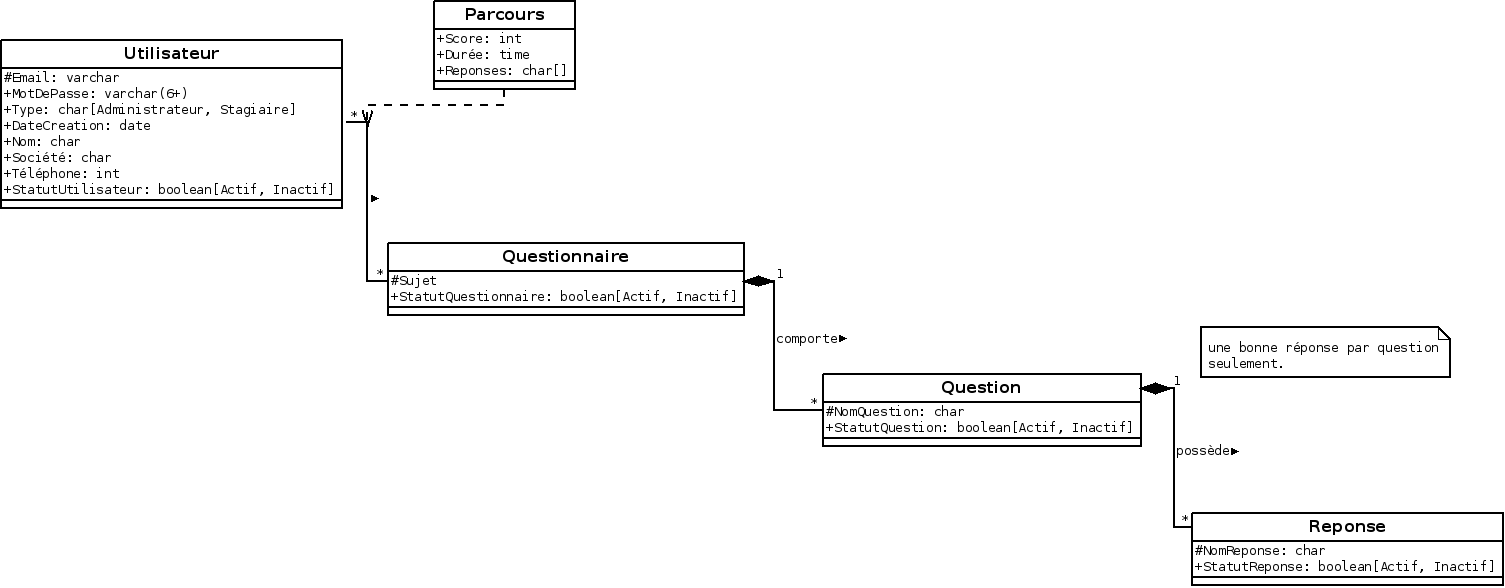
\includegraphics[width=400px]{../model/Modele.png}
		\caption{diagramme UML (incomplet)}
	\end{figure}
\end{center}

\vspace{1cm}

Nous allons dans un premier temps présenter la gestion des utilisateurs. Nous allons ensuite présenter la gestion des questionnaires, puis nous terminerons par la gestion du parcours de l'utilisateur.

\section{Gestion des utilisateurs}
\section{Gestion des questionnaires}
\section{Gestion du parcours}

\end{document}